254. На рисунке показана полоска $2\times 8,$ её периметр равен 20. Если удалить клетки A и C или B и C, то она развалится на части, а если удалить клетки A и B, то периметр оставшейся части станет равен 22. Сколько есть способов удалить из полоски $2\times 20$ две клетки так, чтобы она осталась целой, а периметр оставшейся части был равен 48?
\begin{figure}[ht!]
\center{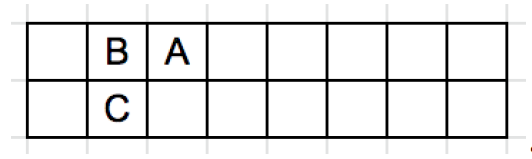
\includegraphics[scale=0.35]{05.png}}
\end{figure}\\
